\documentclass[11pt,letterpaper]{article}
\usepackage[lmargin=1in,rmargin=1in,tmargin=1in,bmargin=1in]{geometry}
\usepackage{../style/homework}
\usepackage{../style/commands}
\setbool{quotetype}{true} % True: Side; False: Under
\setbool{hideans}{false} % Student: True; Instructor: False

% -------------------
% Content
% -------------------
\begin{document}

\homework{7: Due 10/13}{The only function of economic forecasting is to make astrology look respectable.}{John Galbraith}

% Problem 1
\problem{10} As accurately as possible and showing all your work, find the least square regression line, along with the $r$ and $r^2$ value, for the dataset $\{ (1, 0), (0, 1), (1, 1), (2, 6) \}$. Show all your work. \pspace

\sol We have 4 points so that $n= 4$. First, we compute the $x$ and $y$ averages---$\overline{x}$ and $\overline{y}$, respectively. 
	\[
	\begin{aligned}
	\overline{x}&= \dfrac{\sum x_i}{n}= \dfrac{1 + 0 + 1 + 2}{4}= \dfrac{4}{4}= 1 \\
	\overline{y}&= \dfrac{\sum y_i}{n}= \dfrac{0 + 1 + 1 + 6}{4}= \dfrac{8}{4}= 2 
	\end{aligned}
	\]
Now we compute $s_x, s_y, r$:
	\begin{table}[!ht]
	\centering
	\begin{tabular}{rrrrrr}
	$x$ & $y$ & $x_i - \overline{x}$ & $(x_i - \overline{x})^2$ & $y_i - \overline{y}$ & $(y_i - \overline{y})^2$ \\ \hline
	$1$ & $0$ & $0$ & $0$ & $-2$ & $4$ \\ 
	$0$ & $1$ & $-1$ & $1$ & $-1$ & $1$ \\
	$1$ & $1$ & $0$ & $0$ & $-1$ & $1$ \\
	$2$ & $6$ & $1$ & $1$ & $4$ & $16$ \\ \hline
	& Total: & & $2$ & & $22$ 
	\end{tabular}
	\end{table}
Then we have
	\[
	\begin{aligned}
	s_x^2&= \dfrac{1}{n - 1} \sum (x_i - \overline{x})^2= \dfrac{1}{4 - 1} \cdot 2= 0.6667 \Longrightarrow s_x= \sqrt{0.6667}= 0.8165 \\
	s_y^2&= \dfrac{1}{n - 1} \sum (y_i - \overline{y})^2= \dfrac{1}{4 - 1} \cdot 22= 7.3333 \Longrightarrow s_y= \sqrt{7.3333}= 2.7080
	\end{aligned}
	\]
Now we also compute the $r$ value:
	\begin{table}[!ht]
	\centering
	\begin{tabular}{rrrrc}
	$x$ & $y$ & $x_i - \overline{x}$ & $y_i - \overline{y}$ & $(x_i - \overline{x})(y_i - \overline{y})$ \\ \hline
	$1$ & $0$ & $0$ & $-2$ & $0$ \\
	$0$ & $1$ & $-1$ & $-1$ & $1$ \\
	$1$ & $1$ & $0$ & $-1$ & $0$ \\
	$2$ & $6$ & $1$ & $4$ & $4$ \\ \hline
		& 	& 	& Total: & $5$
	\end{tabular}
	\end{table}
	\[
	r= \dfrac{1}{n - 1} \dfrac{1}{s_x s_y} \sum (x_i - \overline{x})(y_i - \overline{y})= \dfrac{1}{4 - 1} \cdot \dfrac{1}{0.8165 \cdot 2.7080} \cdot 5= 0.7537788
	\]
Therefore, $r^2= 0.5682$. Finally, we can compute our regression coefficients:
	\[
	b_1= r\, \dfrac{s_y}{s_x}= 0.7537788 \cdot \dfrac{2.7080}{0.8165}= 2.50 \quad \text{ and } \quad b_0= \overline{y} - b_1 \overline{x}= 2 - 2.50 \cdot 1= -0.5
	\]
Therefore, as $\widehat{y}= b_1x + b_0$, we know $\widehat{y}= 2.50x - 0.5$.  



\newpage



% Problem 2
\problem{10} Given the following information below, find the least square regression line. Show all your work. 
	\[
	\begin{aligned}
	n&= 10 &&& R&= -0.0023 \\
	\overline{x}&= 0.97 &&& \quad s_x^2&= 30.32 \\
	\overline{y}&= -1.33 &&& \quad s_y^2&= 36.54
	\end{aligned}
	\] \pspace

\sol We are given $s_x^2$ and $s_y^2$ so that we have\dots
	\[
	\begin{aligned}
	s_x&= \sqrt{s_x^2}= \sqrt{30.32} \approx 5.50636 \\[0.3cm]
	s_y&= \sqrt{s_y^2}= \sqrt{36.54} \approx 6.04483
	\end{aligned}
	\]
But then we have\dots
	\[
	\begin{aligned}
	b_1&= r \, \dfrac{s_y}{s_x}= -0.0023 \cdot \dfrac{6.04483}{5.50636} \approx -0.00252492 \\[0.3cm]
	b_0&= \overline{y} - b_1 \overline{x}= -1.33 - (-0.00252492) \cdot 0.97= -1.33 - (-0.00244917)= -1.32755083
	\end{aligned}
	\]
Therefore, the model is\dots
	\[
	\widehat{y}= -0.00252492x - 1.32755083
	\]



\newpage



% Problem 3
\problem{10} Match each regression coefficient to its corresponding graph. 
	\begin{figure}[!ht]
	\centering
	\begin{minipage}{0.45\textwidth}
	   \centering
	   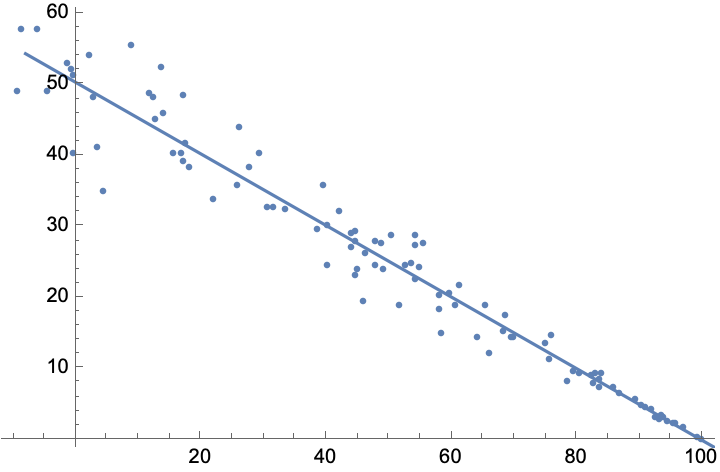
\includegraphics[width=0.9\textwidth]{reg1.png}
	   \caption*{(a)}
	\end{minipage}\hfill
	\begin{minipage}{0.45\textwidth}
	   \centering
	   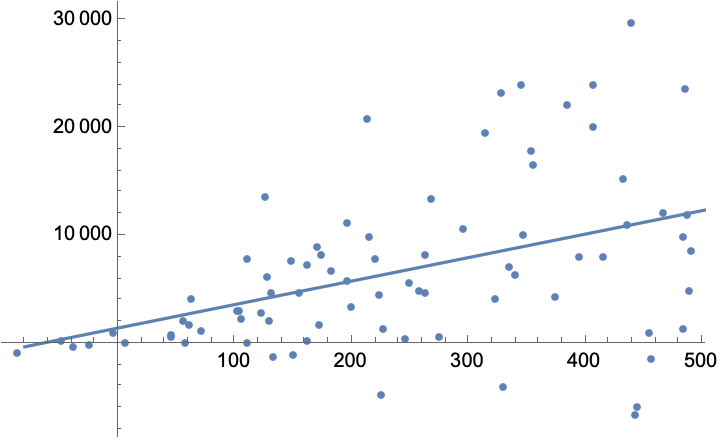
\includegraphics[width=0.9\textwidth]{reg2.png}
	   \caption*{(b)}
	\end{minipage}
	\begin{minipage}{0.45\textwidth}
	   \centering
	   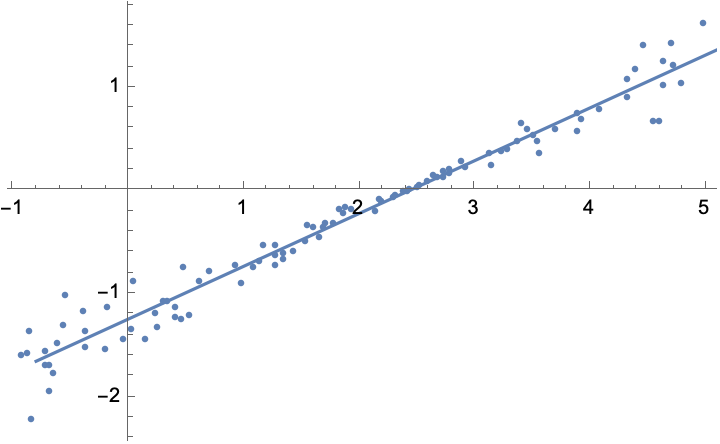
\includegraphics[width=0.9\textwidth]{reg3.png}
	   \caption*{(c)}
	\end{minipage}
	\begin{minipage}{0.45\textwidth}
	   \centering
	   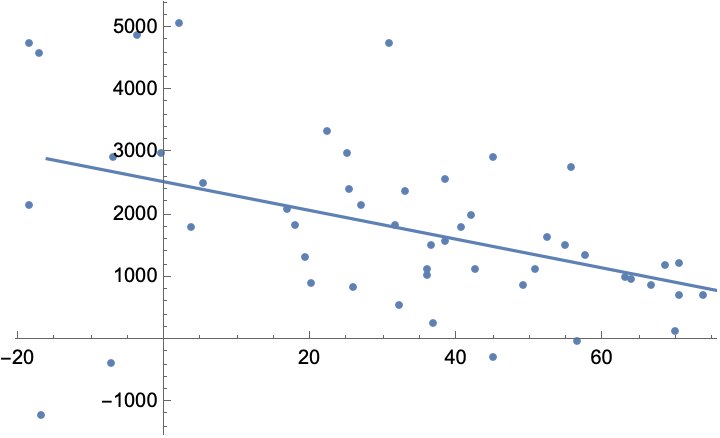
\includegraphics[width=0.9\textwidth]{reg4.png}
	   \caption*{(d)}
	\end{minipage}
	\end{figure}

\begin{enumerate}[(i)]
\item\underline{\hspace{0.5cm}(a)\hspace{0.5cm}}: $R= -0.9197$
\item\underline{\hspace{0.5cm}(d)\hspace{0.5cm}}: $R= -0.6023$
\item\underline{\hspace{0.5cm}(b)\hspace{0.5cm}}: $R= 0.2527$
\item\underline{\hspace{0.5cm}(c)\hspace{0.5cm}}: $R= 0.9616$
\end{enumerate} 



\newpage



% Problem 4
\problem{10} A researcher is predicting penguin weights given their final adult height. They create a linear regression model for the weight of the penguin (in lbs), $W$, given its heigh in cm, $h$. Their model is $W(h)= 0.8h - 56.2$.
	\begin{enumerate}[(a)]
	\item What are $b_0$ and $b_1$ for this linear regression?
	\item How much does a penguin's weight increase per centimeter taller that it is, according to this model?
	\item Does the $y$-intercept for this model hold any meaning? Explain. 
	\item Predict a penguin's weight if its height is 125~cm. Suppose one of the penguins in their dataset has a height of 125~cm and weight of 48.6~lbs. Find the residual for this datapoint. 
	\item The researcher finds an $R^2$ value of $0.4329$. Is this linear model a good predictor of a penguin's weight given its height? Explain. 
	\end{enumerate} \pspace

\sol
\begin{enumerate}[(a)]
\item We know that $b_1$ is the slope of the linear model and $b_0$ is the $y$-intercept of the linear model. Because $W(h)= 0.8h - 56.2$ has slope 0.8 and $y$-intercept $-56.2$, we know that $b_1= 0.8$ and $b_0= -56.2$. \pspace

\item This is the rate of change of the penguin's weight with respect to their height. But this is precisely the slope of the linear model. Because we have $b_1= 0.8= \dfrac{0.8}{1} \leftrightarrow \dfrac{\Delta W}{\Delta h}$. Treating this as $\Delta W= 0.8$ and $\Delta h= 1$, we see that for every additional 1~cm the penguin is in height, the model predicts the penguin's weight increases by 0.8~lbs. \pspace

\item We know that the $y$-intercept occurs when the input is 0. But then we have $W(0)= 0.8(0) - 56.2= 0 - 56.2= -56.2$. Therefore, the $y$-intercept is $(0, -56.2)$. This says that a penguin that is 0~cm tall weighs $-56.2$~lbs. But what is a 0~cm tall penguin? Moreover, what does negative weight mean? Therefore, it is unlikely that the $y$-intercept for this model has an interpretation in the context of the problem. \pspace

\item We have\dots
	\[
	W(125)= 0.8(125) - 56.2= 100.0 - 56.2= 43.8 \text{ lb}
	\]
Therefore, the model predicts that a penguin that is 125~cm tall weighs 43.8~lb. But then the residual, $e_i$, for a penguin that is 125~cm that actually weighs 48.6~lb is $e_i= y - \widehat{y}= 48.6 \text{ lb} - 43.8 \text{ lb}= 4.8 \text{ lb}$. \pspace

\item We know the closer $R^2$ is to 1, the better the model. If $R^2= 1$, then the data is perfectly linear. By `most' standards, $R^2= 0.4329$ is not a good indication that this is a good model. This says that only 43.29\% of the variation in the penguin weight due to height is explained by the model. Typically, we would desire $R^2$ to be greater than 0.60, 0.70, 0.85, 0.95, or 0.99.

\end{enumerate}


\end{document}